\documentclass{article}%文档类型
\usepackage[UTF8]{ctex}%允许中文
\usepackage[a4paper,left=10mm,right=10mm,top=15mm,bottom=15mm]{geometry}%文档布局
\usepackage{titling}%标题包
\usepackage{xcolor}%颜色包
\usepackage{listings}%代码显示包
\usepackage{float}
\usepackage{array}
\usepackage{graphicx}%图像插入包
\usepackage{multirow}
\graphicspath{{../exp/}}
\renewcommand{\arraystretch}{2} % 增加整体行高
\usepackage{appendix}
\usepackage{hyperref}
\usepackage{amsmath}

%代码显示设置
\lstset{
    language=Python, % 设置语言
    basicstyle={\small\ttfamily}, % 设置字体族
    breaklines=true, % 自动换行
    keywordstyle=\color{blue},  % 关键字样式
    commentstyle=\color{green}, % 注释样式
    stringstyle=\color{red},    % 字符串样式
	emph={self},           % 添加强调词
    emphstyle=\color{blue}\bfseries, % 强调词样式
    columns=flexible,
    numbers=left, % 显示行号在左边
    numbersep=2em, % 设置行号的具体位置
    numberstyle=\footnotesize, % 缩小行号
    frame=single, % 边框
    framesep=1em, % 设置代码与边框的距离
	xleftmargin=2em, % 左边距
    xrightmargin=2em, % 右边距
}

\title{视听信息系统导论第二次编程作业报告}

\begin{document}
%标题页
\begin{titlepage}
    \thispagestyle{empty}
    \vspace*{4cm} % 顶部填充
    \begin{center}
    {\LARGE \textbf{\thetitle}}\\
    \vspace{6cm}
    \end{center}
    \vspace*{\fill} % 底部填充
\end{titlepage}

\zihao{-4}
\setlength{\baselineskip}{22pt}
\tableofcontents
\clearpage

\section{实验任务}

\subsection{Task1}
\strong{完成model.py文件中\_\_init\_\_函数。(完成代码即可,不用在报告中写文字说明)}

代码如下:
\begin{lstlisting}
    def __init__(self, in_dim=1280, hidden_dim=256, num_classes=20, \
                roi_output_w=2, roi_output_h=2, drop_ratio=0.3):
        super().__init__()

        assert(num_classes != 0)
        self.num_classes = num_classes
        self.roi_output_w, self.roi_output_h = roi_output_w, roi_output_h
        self.feat_extractor = FeatureExtractor()
        ##############################################################################
        # TODO: Declare the cls & bbox heads (in Fast R-CNN).                        #
        # The cls & bbox heads share a sequential module with a Linear layer,        #
        # followed by a Dropout (p=drop_ratio), a ReLU nonlinearity and another      #
        # Linear layer.                                                              #
        # The cls head is a Linear layer that predicts num_classes + 1 (background). #
        # The det head is a Linear layer that predicts offsets(dim=4).               #
        # HINT: The dimension of the two Linear layers are in_dim -> hidden_dim and  #
        # hidden_dim -> hidden_dim.                                                  #
        ##############################################################################
        # Replace "pass" statement with your code
        self.shared_fc = nn.Sequential(
            nn.Linear(in_dim, hidden_dim),
            nn.Dropout(drop_ratio),
            nn.ReLU(),
            nn.Linear(hidden_dim, hidden_dim)
        )
        self.cls_head = nn.Linear(hidden_dim, num_classes + 1)
        self.bbox_head = nn.Linear(hidden_dim, 4)
        ##############################################################################
        #                               END OF YOUR CODE                             #
        ##############################################################################
\end{lstlisting}

\subsection{Task2}
\strong{完成 utils.py 文件中的 compute\_iou 函数。(完成代码即可,不用在报告中写文字说明)}

代码如下:
\begin{lstlisting}
    def compute_iou(anchors, bboxes):
    """
    Compute the intersection-over-union between anchors and gts.
    
    Inputs:
    - anchors: Anchor boxes, of shape (M, 4), where M is the number of proposals
    - bboxes: GT boxes of shape (N, 4), where N is the number of GT boxes,
                4 indicates (x_{lr}^{gt}, y_{lr}^{gt}, x_{rb}^{gt}, y_{rb}^{gt})
    
    Outputs:
    - iou: IoU matrix of shape (M, N)
    """
    iou = None
    ##############################################################################
    # TODO: Given anchors and gt bboxes,                                         #
    # compute the iou between each anchor and gt bbox.                           #
    ##############################################################################
    x1 = torch.max(anchors[:, None, 0], bboxes[None, :, 0])
    y1 = torch.max(anchors[:, None, 1], bboxes[None, :, 1])
    x2 = torch.min(anchors[:, None, 2], bboxes[None, :, 2])
    y2 = torch.min(anchors[:, None, 3], bboxes[None, :, 3])
    inter = torch.clamp(x2 - x1, min=0) * torch.clamp(y2 - y1, min=0)
    area_anchors = (anchors[:, 2] - anchors[:, 0]) * (anchors[:, 3] - anchors[:, 1])
    area_bboxes = (bboxes[:, 2] - bboxes[:, 0]) * (bboxes[:, 3] - bboxes[:, 1])
    union = area_anchors[:, None] + area_bboxes[None, :] - inter
    iou = torch.zeros_like(union)
    non_zero_union = union > 0
    iou[non_zero_union] = inter[non_zero_union] / union[non_zero_union]
    ##############################################################################
    #                               END OF YOUR CODE                             #
    ##############################################################################

    return iou
\end{lstlisting}

\subsection{Task3}

\strong{阅读 utils.py 文件中的 assign\_label 函数,并简要说明该函数如何判断正负样本框。}

答:assign\_label 函数用于在模型训练中将候选框(proposals)分配为正样本或负样本。
如果某个候选框与任意一个 GT 框的 IoU 值是所有候选框中的最大值,或者当候选框与某个 GT 框的 IoU 大于正样本阈值(pos\_thresh)时,则该候选框被标记为正样本。
当候选框与所有 GT 框的 IoU 值都小于负样本阈值(neg\_thresh)时,该候选框被标记为负样本,此外再随机采样负样本以平衡正负比例。

\strong{阅读 utils.py 文件中的 compute\_offsets 函数,简要说明如何计算正样本框到真实框的偏移量。}

答:compute\_offsets 函数用于计算正样本框(anchors)相对于真实框(GT boxes)的偏移量,以便在模型训练中进行位置调整。

计算 GT 框和 anchor 框的宽高比例,通过 torch.log 函数取对数来得到宽高偏移量:

\begin{equation}
    \Delta w = \log\left(\frac{w^{\text{gt}}}{w^{\text{anchor}}}\right), \quad \Delta h = \log\left(\frac{h^{\text{gt}}}{h^{\text{anchor}}}\right)
\end{equation}

计算 GT 框与 anchor 框的中心坐标差异,并对 anchor 框的宽高进行归一化来得到中心坐标偏移量:

\begin{equation}
    \Delta x = \frac{x_{\text{center}}^{\text{gt}} - x_{\text{center}}^{\text{anchor}}}{w^{\text{anchor}}}, \quad \Delta y = \frac{y_{\text{center}}^{\text{gt}} - y_{\text{center}}^{\text{anchor}}}{h^{\text{anchor}}}
\end{equation}

随后将这四个偏移量拼接在一起,得到最终的偏移量。

\begin{equation}
    \text{offsets} = (\Delta x, \Delta y, \Delta w, \Delta h)
\end{equation}

\subsection{Task4}
\strong{完成 model.py 文件中的 forward 函数。(完成代码即可,不用在报告中写文字说明)}

代码如下:
\begin{lstlisting}
    def forward(self, images, bboxes, bbox_batch_ids, proposals, proposal_batch_ids):
        """
        Training-time forward pass for our two-stage Faster R-CNN detector.

        Inputs:
        - images: Tensor of shape (B, 3, H, W) giving input images
        - bboxes: Tensor of shape (N, 5) giving ground-truth bounding boxes
        and category labels, from the dataloader, where N is the total number
        of GT boxes in the batch
        - bbox_batch_ids: Tensor of shape (N, ) giving the index (in the batch)
        of the image that each GT box belongs to
        - proposals: Tensor of shape (M, 4) giving the proposals for input images, 
        where M is the total number of proposals in the batch
        - proposal_batch_ids: Tensor of shape (M, ) giving the index of the image 
        that each proposals belongs to

        Outputs:
        - total_loss: Torch scalar giving the overall training loss.
        """
        w_cls = 1 # for cls_scores
        w_bbox = 1 # for offsets
        total_loss = None
        ##############################################################################
        # TODO: Implement the forward pass of Fast R-CNN.                            #
        # A few key steps are outlined as follows:                                   #
        # i) Extract image fearure.                                                  #
        # ii) Perform RoI Align on proposals, then meanpool the feature in the       #
        #     spatial dimension.                                                     #
        # iii) Pass the RoI feature through the shared-fc layer. Predict             #
        #      classification scores ans box offsets.                                #
        # iv) Assign the proposals with targets of each image.                       # 
        # v) Compute the cls_loss between the predicted class_prob and GT_class      #
        #    (For poistive & negative proposals)                                     #
        #    Compute the bbox_loss between the offsets and GT_offsets                #
        #    (For positive proposals)                                                #
        #    Compute the total_loss which is formulated as:                          #
        #    total_loss = w_cls*cls_loss + w_bbox*bbox_loss.                         #
        ##############################################################################
        # Replace "pass" statement with your code
        B, _, H, W = images.shape
        
        # extract image feature
        features = self.feat_extractor(images)

        # perform RoI Pool & mean pool
        boxes = torch.cat((proposal_batch_ids.unsqueeze(1), proposals), dim=-1)
        roi_feat = torchvision.ops.roi_pool(features, boxes, (self.roi_output_w, self.roi_output_h))
        roi_feat = roi_feat.mean(dim=[2, 3])

        # forward heads, get predicted cls scores & offsets
        shared_feat = self.shared_fc(roi_feat)
        cls_scores = self.cls_head(shared_feat)
        bbox_offsets = self.bbox_head(shared_feat)

        # assign targets with proposals
        pos_masks, neg_masks, GT_labels, GT_bboxes = [], [], [], []
        for img_idx in range(B):
            # get the positive/negative proposals and corresponding
            # GT box & class label of this image
            proposals_img = proposals[proposal_batch_ids == img_idx]
            bboxes_img = bboxes[bbox_batch_ids == img_idx]
            pos_mask, neg_mask, GT_label, GT_bbox = assign_label(proposals_img, bboxes_img, self.num_classes)
            pos_masks.append(pos_mask)
            neg_masks.append(neg_mask)
            GT_labels.append(GT_label)
            GT_bboxes.append(GT_bbox)

        # compute loss
        cls_loss = 0
        bbox_loss = 0
        for img_idx in range(B):
            pos_mask = pos_masks[img_idx]
            neg_mask = neg_masks[img_idx]
            GT_label = GT_labels[img_idx]
            GT_bbox = GT_bboxes[img_idx]
            proposals_img = proposals[proposal_batch_ids == img_idx]
            cls_scores_img = cls_scores[proposal_batch_ids == img_idx]
            bbox_offsets_img = bbox_offsets[proposal_batch_ids == img_idx]
            cls_loss += ClsScoreRegression(cls_scores_img[pos_mask | neg_mask], GT_label[pos_mask | neg_mask], B)
            bbox_loss += BboxRegression(bbox_offsets_img[pos_mask], compute_offsets(proposals_img[pos_mask], GT_bbox), B)
        total_loss = w_cls * cls_loss + w_bbox * bbox_loss
        ##############################################################################
        #                               END OF YOUR CODE                             #
        ##############################################################################
        return total_loss
\end{lstlisting}

\subsection{Task5}
\strong{完成 utils.py 的 generate\_proposal 函数。(完成代码即可,不用在报告中写文字说明)}

代码如下:
\begin{lstlisting}
    def generate_proposal(anchors, offsets):
    """
    Proposal generator.

    Inputs:
    - anchors: Anchor boxes, of shape (M, 4). Anchors are represented
    by the coordinates of their top-left and bottom-right corners.
    - offsets: Transformations of shape (M, 4) that will be used to
    convert anchor boxes into region proposals. The transformation
    offsets[m] = (tx, ty, tw, th) will be applied to the anchor
    anchors[m].

    Outputs:
    - proposals: Region proposals of shape (M, 4), represented by the
    coordinates of their top-left and bottom-right corners. Applying the
    transform offsets[m] to the anchor[m] should give the
    proposal proposals[m].

    """
    proposals = None
    ##############################################################################
    # TODO: Given anchor coordinates and the proposed offset for each anchor,    #
    # compute the proposal coordinates using the transformation formulas above.  #
    ##############################################################################
    # Replace "pass" statement with your code
    xy_offsets = offsets[:, :2]
    wh_offsets = offsets[:, 2:4]
    proposals_minus = torch.exp(wh_offsets) * (anchors[:, 2:4] - anchors[:, :2])
    proposals_plus = xy_offsets * (anchors[:, 2:4] - anchors[:, :2]) * 2 + (anchors[:, :2] + anchors[:, 2:4])
    proposals = torch.cat(((proposals_plus - proposals_minus) / 2, (proposals_plus + proposals_minus) / 2), dim=-1)
    ##############################################################################
    #                               END OF YOUR CODE                             #
    ##############################################################################

    return proposals
\end{lstlisting}

\subsection{Task6}
\strong{完成 model.py 的 inference 函数。(完成代码即可,不用在报告中写文字说明)}

代码如下:
\begin{lstlisting}
    def inference(self, images, proposals, proposal_batch_ids, thresh=0.5, nms_thresh=0.7):
        """"
        Inference-time forward pass for our two-stage Faster R-CNN detector

        Inputs:
        - images: Tensor of shape (B, 3, H, W) giving input images
        - proposals: Tensor of shape (M, 4) giving the proposals for input images, 
        where M is the total number of proposals in the batch
        - proposal_batch_ids: Tensor of shape (M, ) giving the index of the image 
        that each proposals belongs to
        - thresh: Threshold value on confidence probability. HINT: You can convert the
        classification score to probability using a softmax nonlinearity.
        - nms_thresh: IoU threshold for NMS

        We can output a variable number of predicted boxes per input image.
        In particular we assume that the input images[i] gives rise to P_i final
        predicted boxes.

        Outputs:
        - final_proposals: List of length (B,) where final_proposals[i] is a Tensor
        of shape (P_i, 4) giving the coordinates of the final predicted boxes for
        the input images[i]
        - final_conf_probs: List of length (B,) where final_conf_probs[i] is a
        Tensor of shape (P_i, 1) giving the predicted probabilites that the boxes
        in final_proposals[i] are objects (vs background)
        - final_class: List of length (B,), where final_class[i] is an int64 Tensor
        of shape (P_i, 1) giving the predicted category labels for each box in
        final_proposals[i].
        """
        final_proposals, final_conf_probs, final_class = None, None, None
        ##############################################################################
        # TODO: Predicting the final proposal coordinates `final_proposals`,         #
        # confidence scores `final_conf_probs`, and the class index `final_class`.   #
        # The overall steps are similar to the forward pass, but now you cannot      #
        # decide the activated nor negative proposals without GT boxes.              #
        # You should apply post-processing (thresholding and NMS) to all proposals   #
        # and keep the final proposals.                                               #
        ##############################################################################
        # Replace "pass" statement with your code
        B = images.shape[0]

        # extract image feature
        features = self.feat_extractor(images)

        # perform RoI Pool & mean pool
        boxes = torch.cat((proposal_batch_ids.unsqueeze(1), proposals), dim=-1)
        roi_feat = torchvision.ops.roi_pool(features, boxes, (self.roi_output_w, self.roi_output_h))
        roi_feat = roi_feat.mean(dim=[2, 3])

        # forward heads, get predicted cls scores & offsets
        shared_feat = self.shared_fc(roi_feat)
        cls_scores = self.cls_head(shared_feat)
        bbox_offsets = self.bbox_head(shared_feat)

        # get predicted boxes & class label & confidence probability
        conf_probs = torch.softmax(cls_scores, dim=-1)
        pred_boxes = generate_proposal(proposals, bbox_offsets)

        final_proposals = []
        final_conf_probs = []
        final_class = []
        # post-process to get final predictions
        for img_idx in range(B):

            # filter by threshold
            img_proposals = pred_boxes[proposal_batch_ids == img_idx]
            img_conf_probs = conf_probs[proposal_batch_ids == img_idx]
            img_cls_scores = cls_scores[proposal_batch_ids == img_idx]
            keep = img_conf_probs[:, :self.num_classes].max(dim=1).values > thresh
            img_proposals = img_proposals[keep]
            img_conf_probs = img_conf_probs[keep]
            img_cls_scores = img_cls_scores[keep]
            conf_values, pred_classes = img_conf_probs[:, :self.num_classes].max(dim=1)

            # nms
            keep_idx = torchvision.ops.nms(img_proposals, conf_values, nms_thresh)
            final_proposals.append(img_proposals[keep_idx])
            final_conf_probs.append(conf_values[keep_idx].unsqueeze(1))
            final_class.append(pred_classes[keep_idx].unsqueeze(1))

        ##############################################################################
        #                               END OF YOUR CODE                             #
        ##############################################################################
        return final_proposals, final_conf_probs, final_class
\end{lstlisting}

\subsection{Task7}
\strong{完成过拟合实验,在报告中给出训练损失曲线和测试样本可视化。}

训练损失函数曲线和测试样本可视化如下:
\begin{figure}[H]
	\centering
    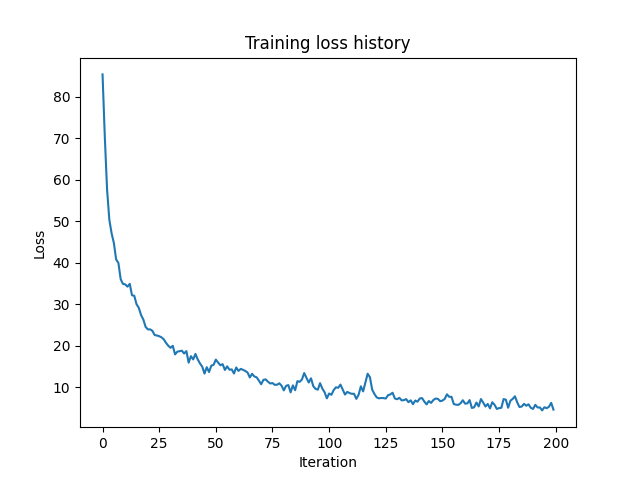
\includegraphics[width=0.7\linewidth]{fast_rcnn_overfit_small/training_loss.png}
    \caption{训练损失曲线}
\end{figure}

\begin{figure}[H]
    \centering
	\begin{minipage}{0.32\linewidth}
		\centering
		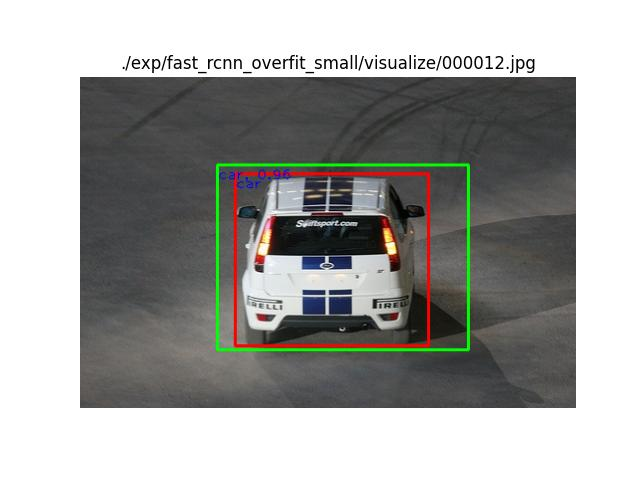
\includegraphics[width=0.9\linewidth]{fast_rcnn_overfit_small/visualize/000012.jpg}
	\end{minipage}
	\begin{minipage}{0.32\linewidth}
		\centering
		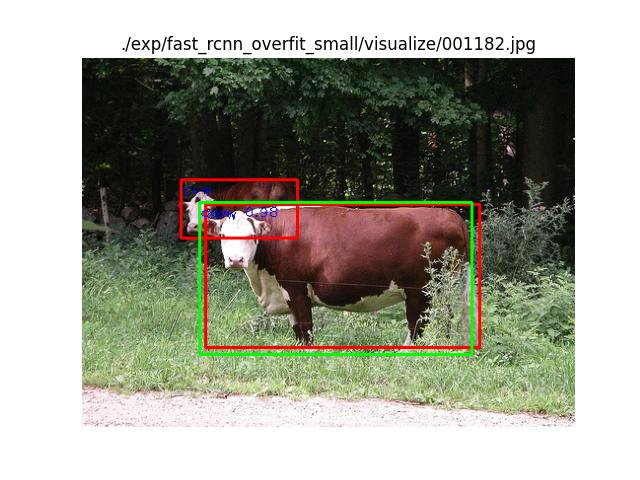
\includegraphics[width=0.9\linewidth]{fast_rcnn_overfit_small/visualize/001182.jpg}
	\end{minipage}
    \begin{minipage}{0.32\linewidth}
		\centering
		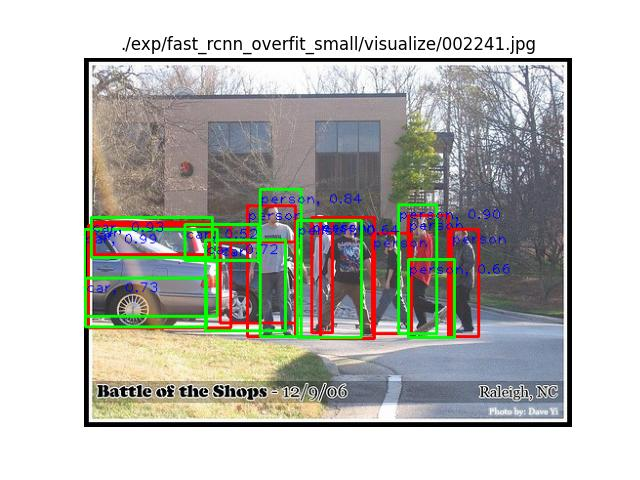
\includegraphics[width=0.9\linewidth]{fast_rcnn_overfit_small/visualize/002241.jpg}
	\end{minipage}
\end{figure}

\begin{figure}[H]
    \centering
	\begin{minipage}{0.32\linewidth}
		\centering
		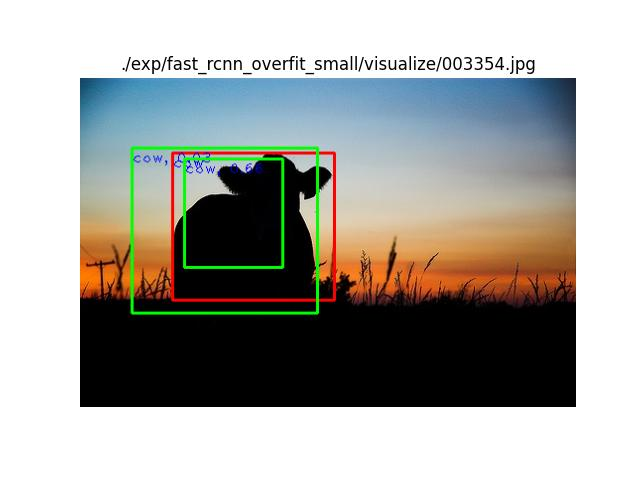
\includegraphics[width=0.9\linewidth]{fast_rcnn_overfit_small/visualize/003354.jpg}
	\end{minipage}
	\begin{minipage}{0.32\linewidth}
		\centering
		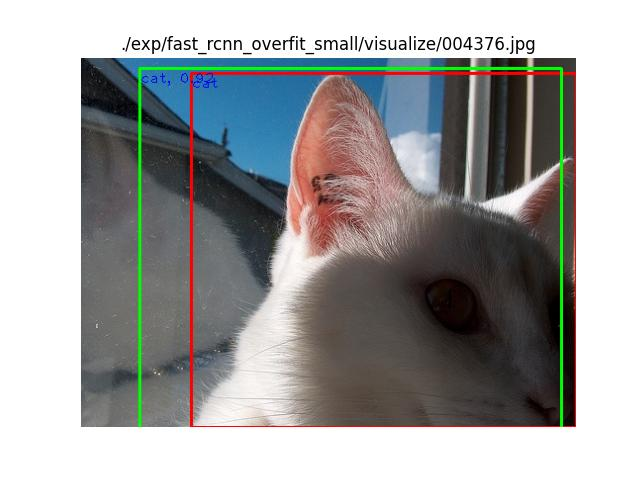
\includegraphics[width=0.9\linewidth]{fast_rcnn_overfit_small/visualize/004376.jpg}
	\end{minipage}
    \begin{minipage}{0.32\linewidth}
		\centering
		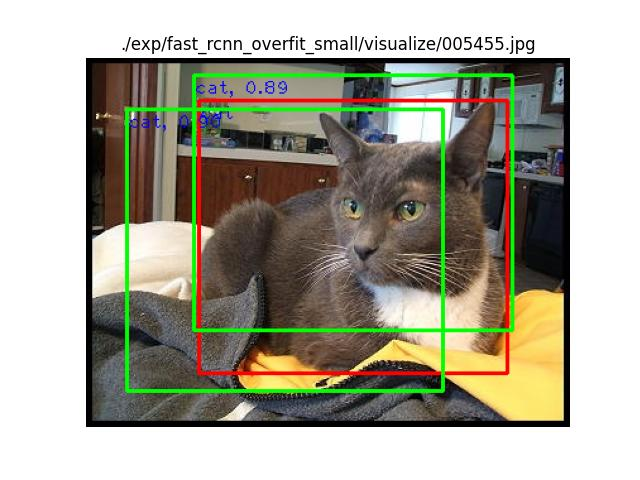
\includegraphics[width=0.9\linewidth]{fast_rcnn_overfit_small/visualize/005455.jpg}
	\end{minipage}
\end{figure}

\begin{figure}[H]
    \centering
	\begin{minipage}{0.32\linewidth}
		\centering
		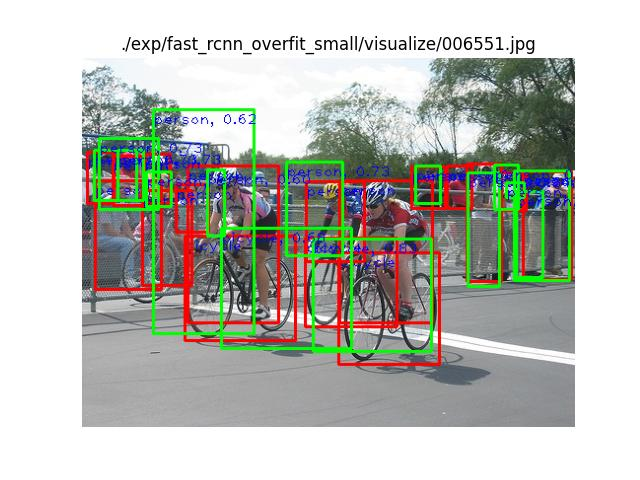
\includegraphics[width=0.9\linewidth]{fast_rcnn_overfit_small/visualize/006551.jpg}
	\end{minipage}
	\begin{minipage}{0.32\linewidth}
		\centering
		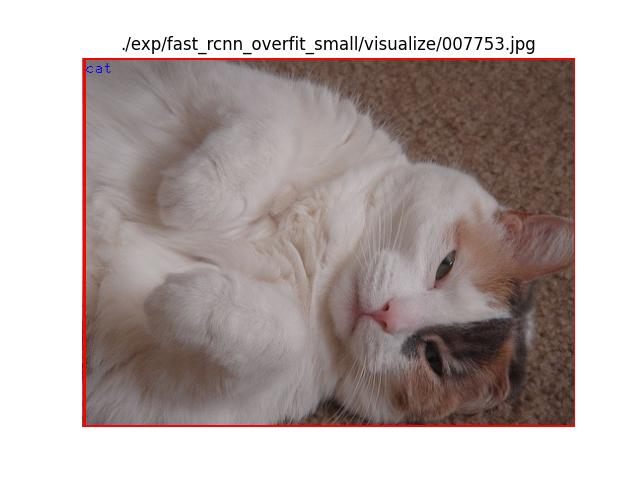
\includegraphics[width=0.9\linewidth]{fast_rcnn_overfit_small/visualize/007753.jpg}
	\end{minipage}
    \begin{minipage}{0.32\linewidth}
		\centering
		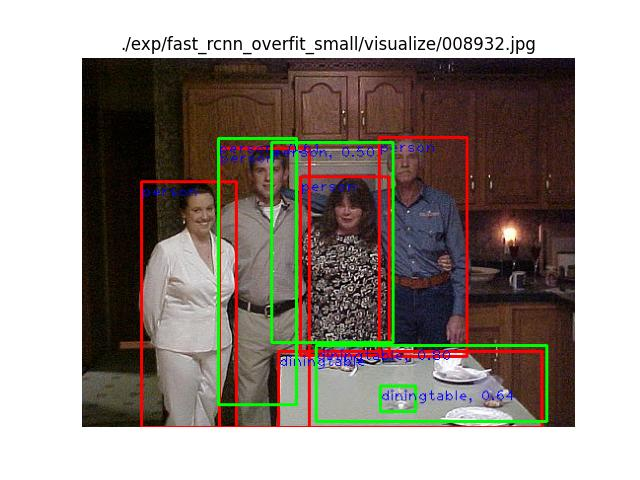
\includegraphics[width=0.9\linewidth]{fast_rcnn_overfit_small/visualize/008932.jpg}
	\end{minipage}
\end{figure}

\begin{figure}[H]
    \centering
	\begin{minipage}{0.32\linewidth}
		\centering
		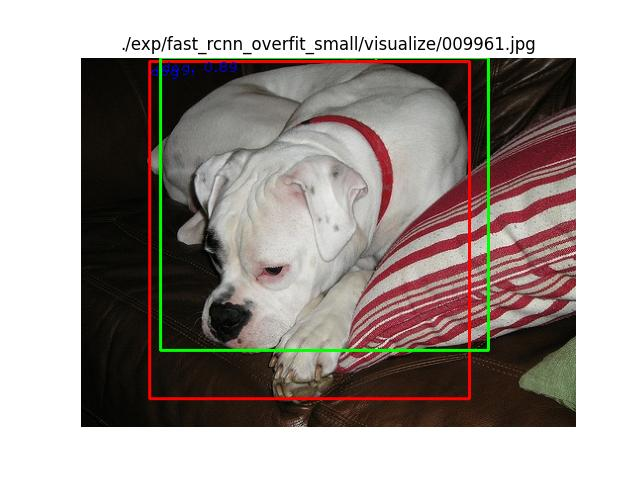
\includegraphics[width=0.9\linewidth]{fast_rcnn_overfit_small/visualize/009961.jpg}
	\end{minipage}
\end{figure}

注意到,训练损失函数曲线和“car”的测试样本与说明文档中的示例几乎完全一致,说明实验结果符合预期。

\subsection{Task8}
\strong{完成最终实验,在报告中给出训练损失曲线和评测情况。}

训练损失曲线和评测情况如下:
\begin{figure}[H]
	\centering
    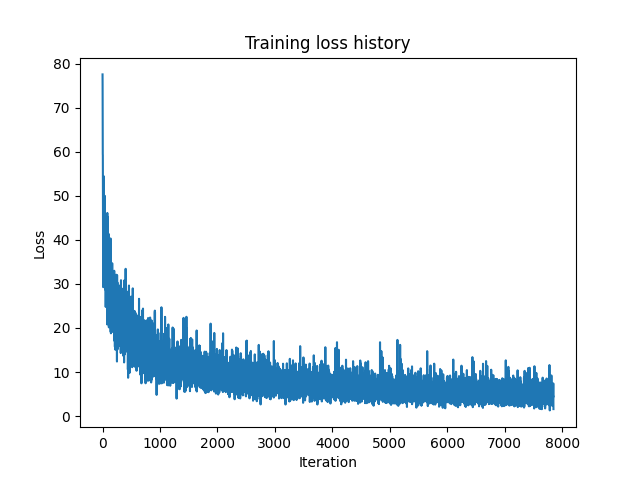
\includegraphics[width=0.7\linewidth]{fast_rcnn/training_loss.png}
    \caption{最终训练损失曲线}
\end{figure}
\begin{figure}[H]
    \centering
	\begin{minipage}{0.49\linewidth}
		\centering
		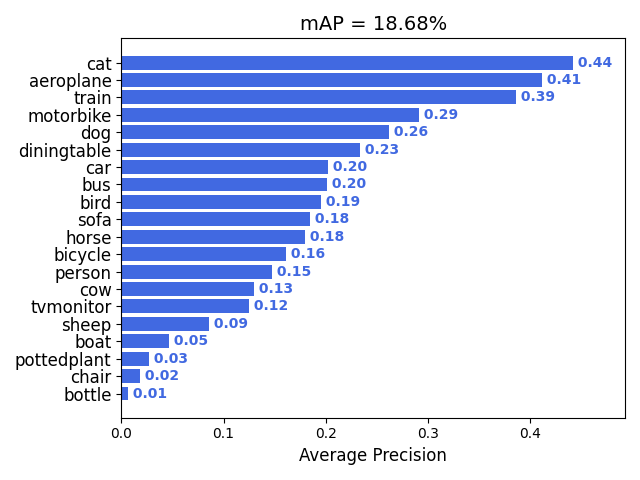
\includegraphics[width=0.9\linewidth]{fast_rcnn/mAP_output/mAP.png}
	\end{minipage}
	\begin{minipage}{0.49\linewidth}
		\centering
		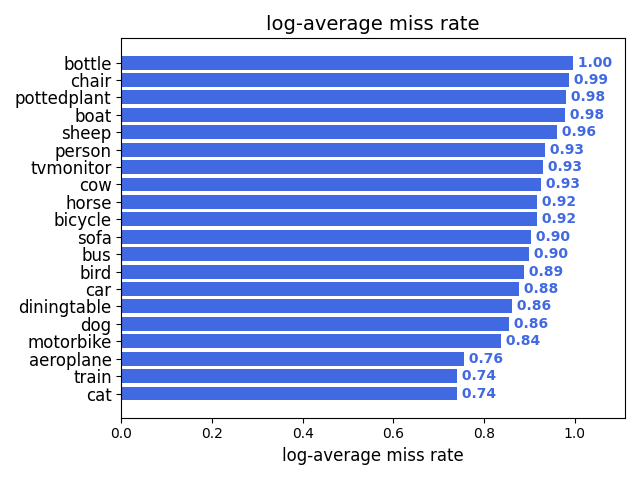
\includegraphics[width=0.9\linewidth]{fast_rcnn/mAP_output/lamr.png}
	\end{minipage}
\end{figure}
\begin{figure}[H]
    \centering
	\begin{minipage}{0.49\linewidth}
		\centering
		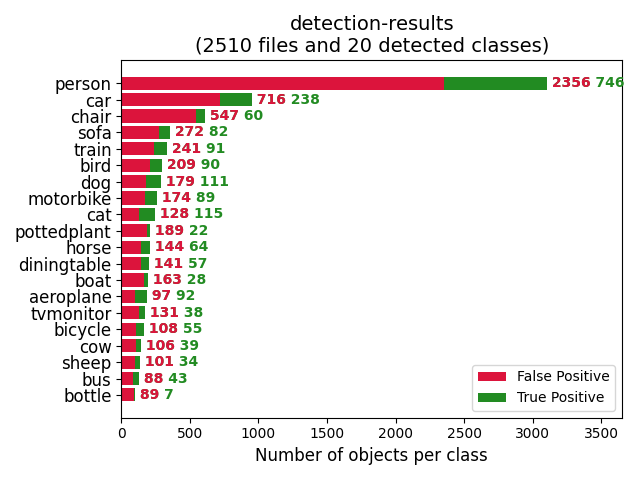
\includegraphics[width=0.9\linewidth]{fast_rcnn/mAP_output/detection-results-info.png}
	\end{minipage}
	\begin{minipage}{0.49\linewidth}
		\centering
		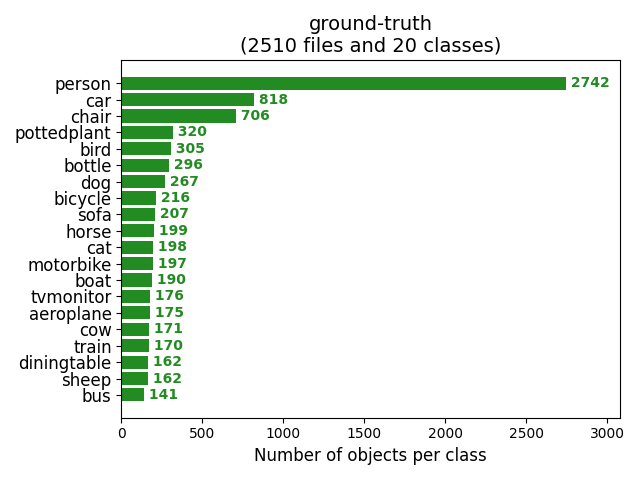
\includegraphics[width=0.9\linewidth]{fast_rcnn/mAP_output/ground-truth-info.png}
	\end{minipage}
\end{figure}
\begin{figure}[H]
    \centering
	\begin{minipage}{0.24\linewidth}
		\centering
		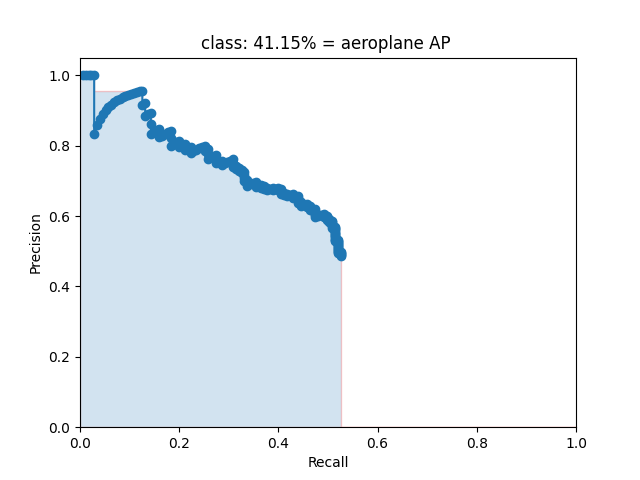
\includegraphics[width=0.9\linewidth]{fast_rcnn/mAP_output/classes/aeroplane.png}
	\end{minipage}
	\begin{minipage}{0.24\linewidth}
		\centering
		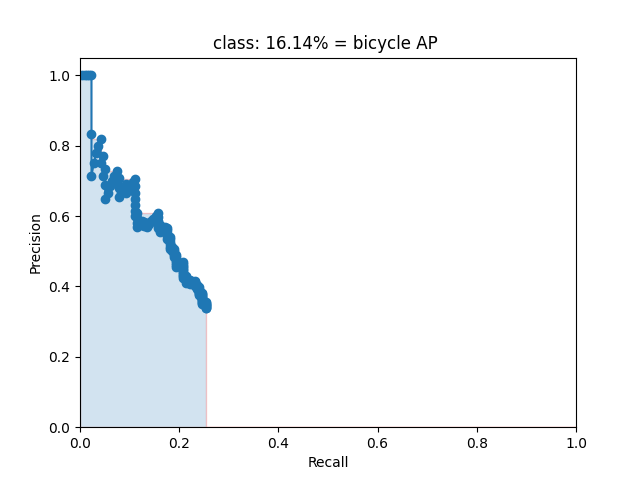
\includegraphics[width=0.9\linewidth]{fast_rcnn/mAP_output/classes/bicycle.png}
	\end{minipage}
    \begin{minipage}{0.24\linewidth}
		\centering
		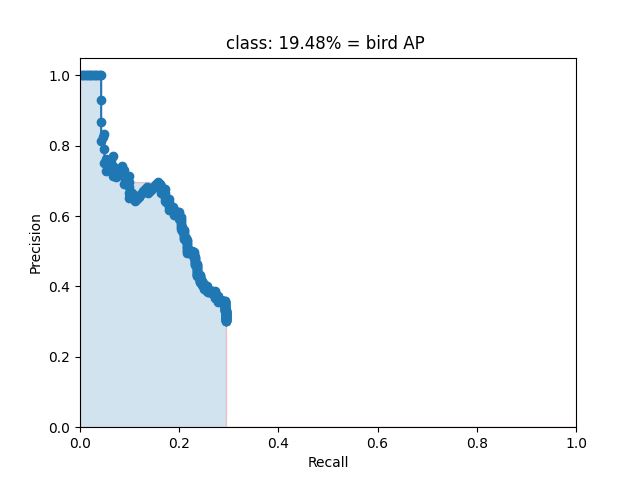
\includegraphics[width=0.9\linewidth]{fast_rcnn/mAP_output/classes/bird.png}
	\end{minipage}
    \begin{minipage}{0.24\linewidth}
		\centering
		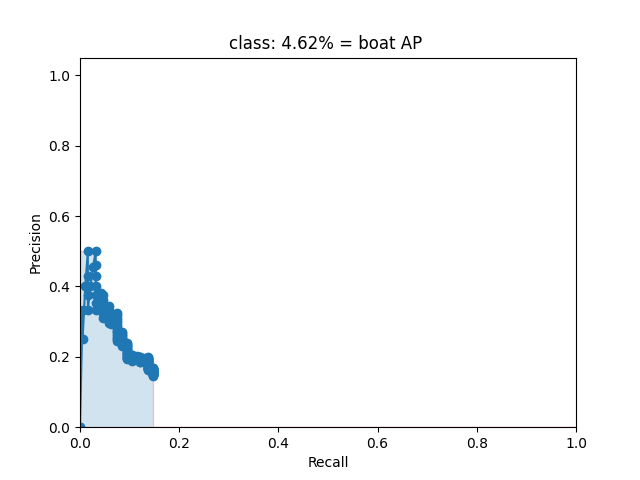
\includegraphics[width=0.9\linewidth]{fast_rcnn/mAP_output/classes/boat.png}
	\end{minipage}
\end{figure}
\begin{figure}[H]
    \centering
	\begin{minipage}{0.24\linewidth}
		\centering
		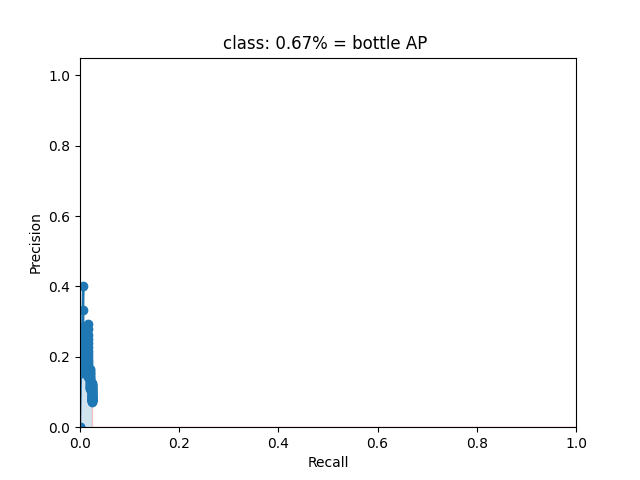
\includegraphics[width=0.9\linewidth]{fast_rcnn/mAP_output/classes/bottle.png}
	\end{minipage}
	\begin{minipage}{0.24\linewidth}
		\centering
		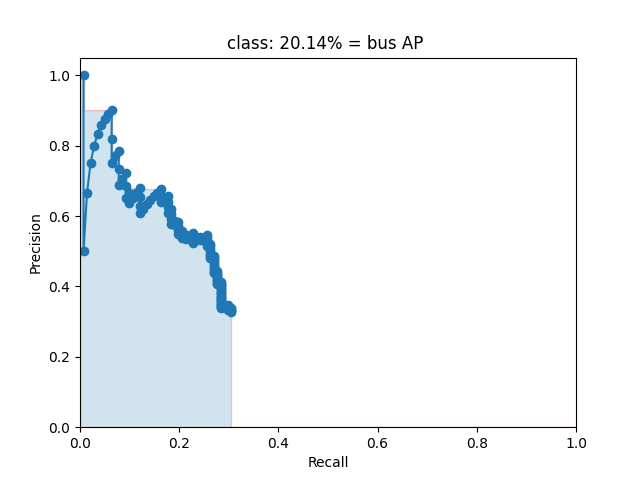
\includegraphics[width=0.9\linewidth]{fast_rcnn/mAP_output/classes/bus.png}
	\end{minipage}
    \begin{minipage}{0.24\linewidth}
		\centering
		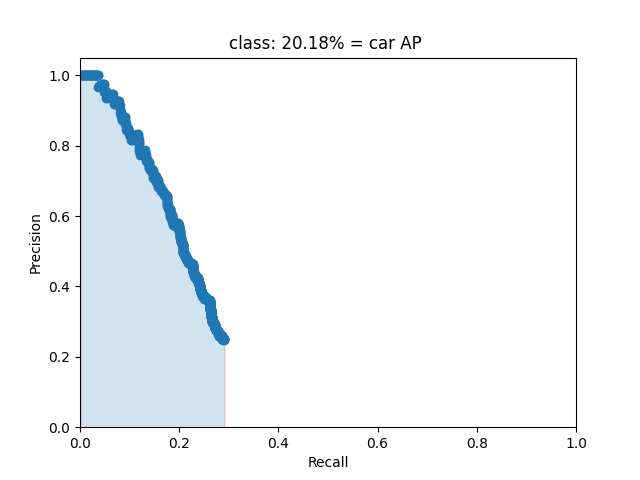
\includegraphics[width=0.9\linewidth]{fast_rcnn/mAP_output/classes/car.png}
	\end{minipage}
    \begin{minipage}{0.24\linewidth}
		\centering
		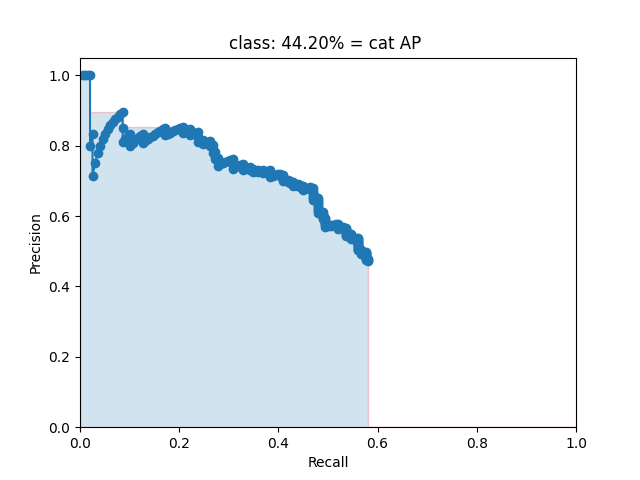
\includegraphics[width=0.9\linewidth]{fast_rcnn/mAP_output/classes/cat.png}
	\end{minipage}
\end{figure}
\begin{figure}[H]
    \centering
	\begin{minipage}{0.24\linewidth}
		\centering
		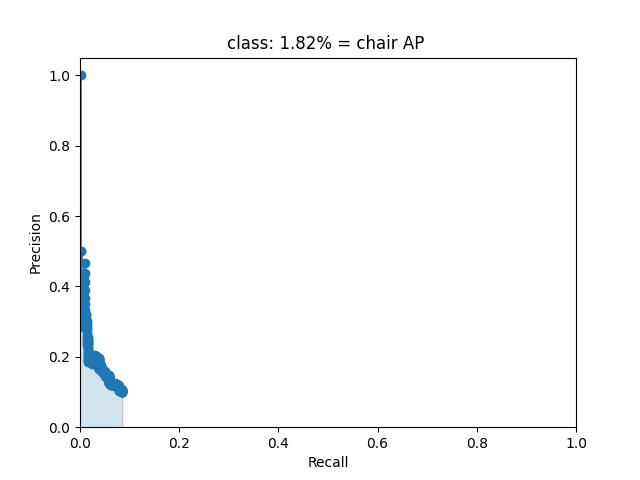
\includegraphics[width=0.9\linewidth]{fast_rcnn/mAP_output/classes/chair.png}
	\end{minipage}
	\begin{minipage}{0.24\linewidth}
		\centering
		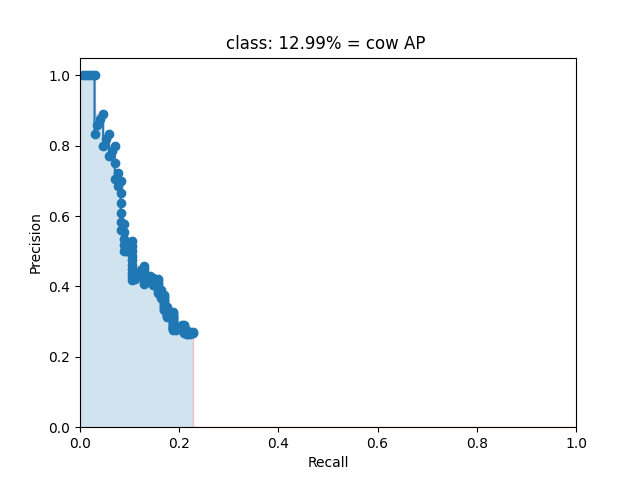
\includegraphics[width=0.9\linewidth]{fast_rcnn/mAP_output/classes/cow.png}
	\end{minipage}
    \begin{minipage}{0.24\linewidth}
		\centering
		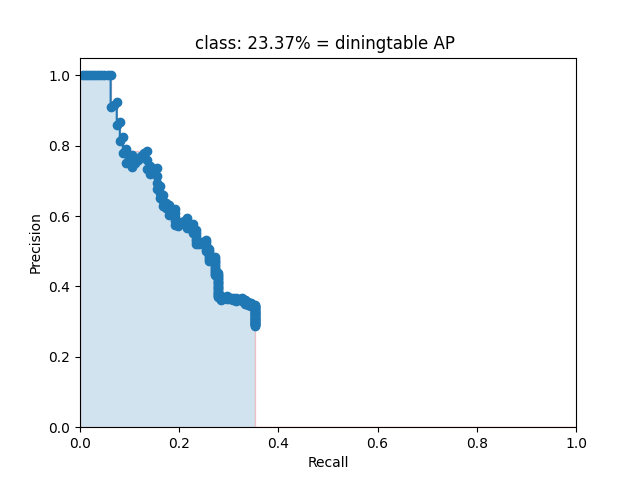
\includegraphics[width=0.9\linewidth]{fast_rcnn/mAP_output/classes/diningtable.png}
	\end{minipage}
    \begin{minipage}{0.24\linewidth}
		\centering
		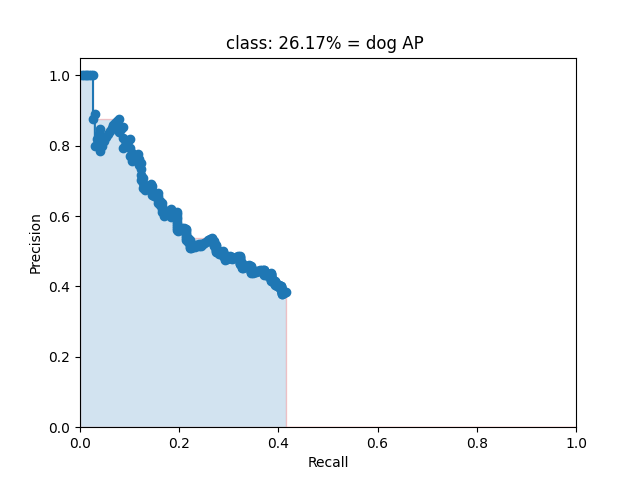
\includegraphics[width=0.9\linewidth]{fast_rcnn/mAP_output/classes/dog.png}
	\end{minipage}
\end{figure}
\begin{figure}[H]
    \centering
	\begin{minipage}{0.24\linewidth}
		\centering
		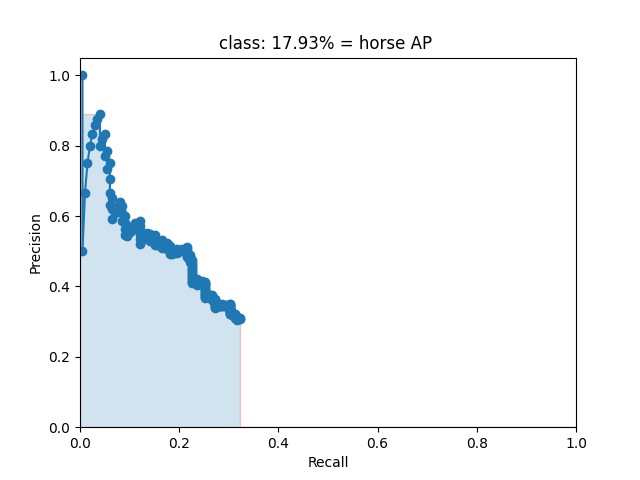
\includegraphics[width=0.9\linewidth]{fast_rcnn/mAP_output/classes/horse.png}
	\end{minipage}
	\begin{minipage}{0.24\linewidth}
		\centering
		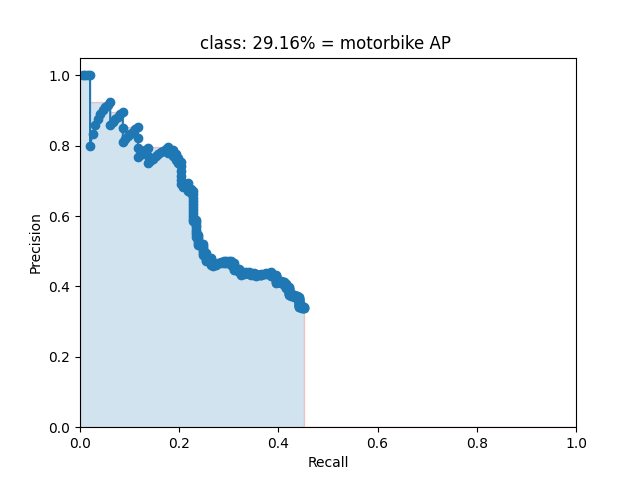
\includegraphics[width=0.9\linewidth]{fast_rcnn/mAP_output/classes/motorbike.png}
	\end{minipage}
    \begin{minipage}{0.24\linewidth}
		\centering
		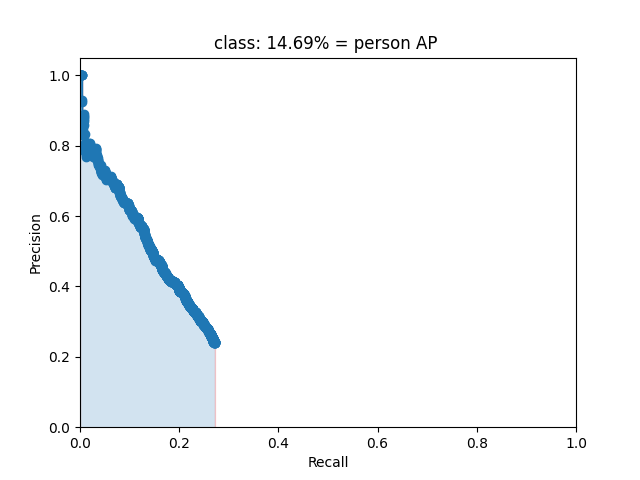
\includegraphics[width=0.9\linewidth]{fast_rcnn/mAP_output/classes/person.png}
	\end{minipage}
    \begin{minipage}{0.24\linewidth}
		\centering
		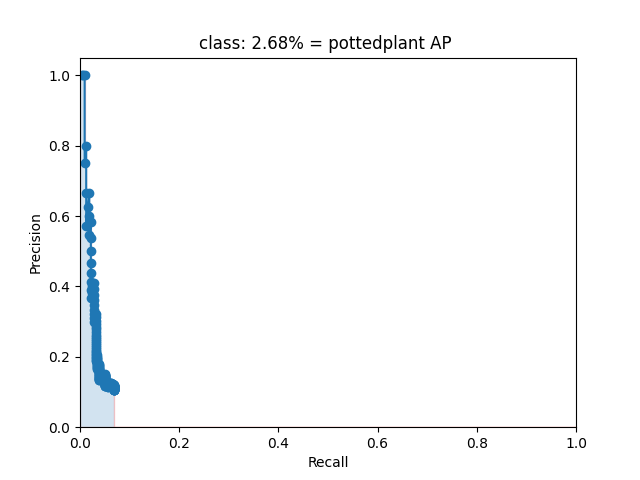
\includegraphics[width=0.9\linewidth]{fast_rcnn/mAP_output/classes/pottedplant.png}
	\end{minipage}
\end{figure}
\begin{figure}[H]
    \centering
	\begin{minipage}{0.24\linewidth}
		\centering
		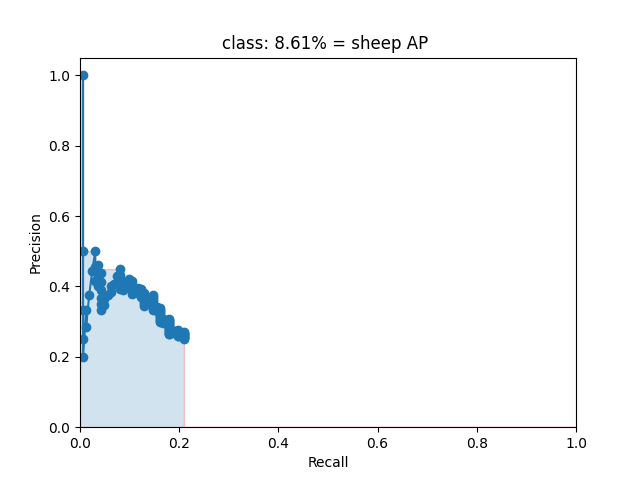
\includegraphics[width=0.9\linewidth]{fast_rcnn/mAP_output/classes/sheep.png}
	\end{minipage}
	\begin{minipage}{0.24\linewidth}
		\centering
		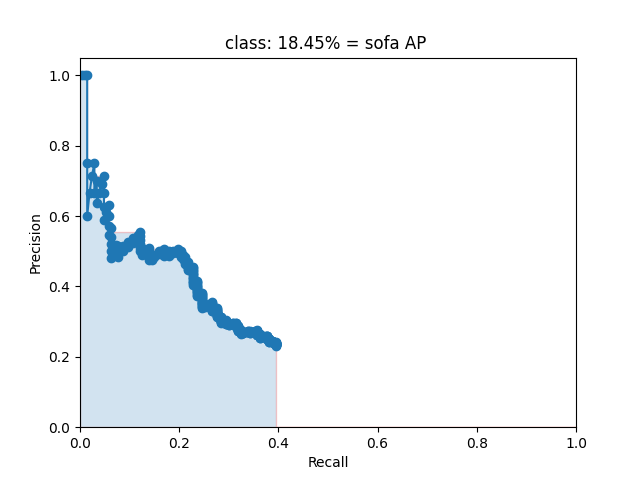
\includegraphics[width=0.9\linewidth]{fast_rcnn/mAP_output/classes/sofa.png}
	\end{minipage}
    \begin{minipage}{0.24\linewidth}
		\centering
		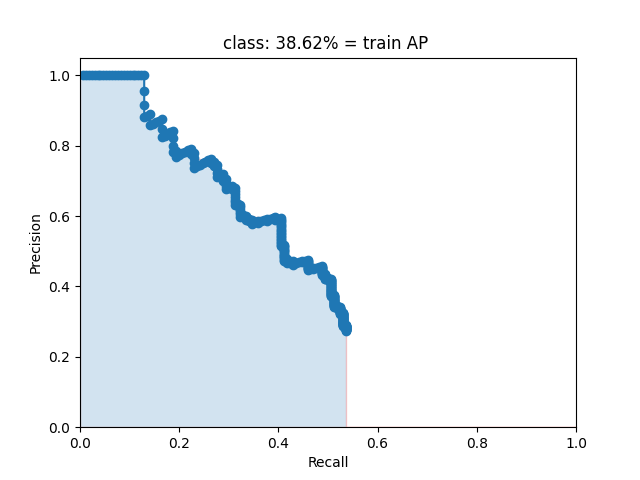
\includegraphics[width=0.9\linewidth]{fast_rcnn/mAP_output/classes/train.png}
	\end{minipage}
    \begin{minipage}{0.24\linewidth}
		\centering
		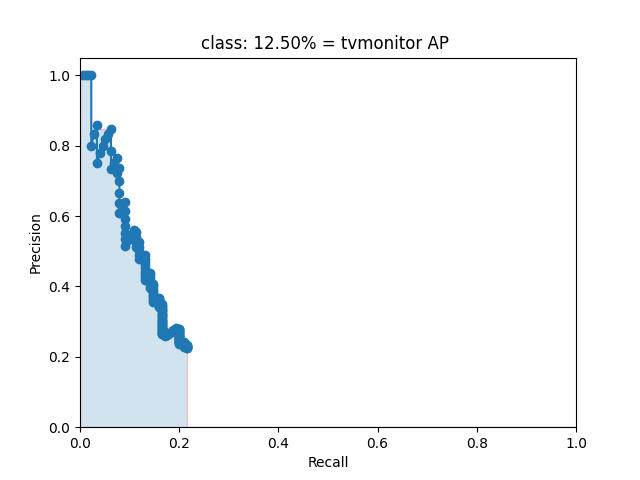
\includegraphics[width=0.9\linewidth]{fast_rcnn/mAP_output/classes/tvmonitor.png}
	\end{minipage}
\end{figure}

受限于算力和时间,最终评测得到的 mAP 为 18.68\%,与说明文档中的预期(18\% 左右)相符。

\end{document}
